El diagrama muestra un triángulo rectángulo y tres cuadrados.
El área del cuadrado más grande es 67 unidades$^2$, como se muestra en la figura \ref{fig:area12}.
\begin{figure}[H]
    \begin{center}
        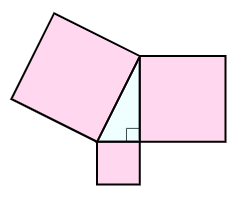
\includegraphics[width=0.4\textwidth]{../images/area12.png}
    \end{center}
    \caption{}
    \label{fig:area12}
\end{figure}

\begin{parts}
    \part \textbf{¿Cuáles pueden ser las áreas de los cuadrados más pequeños?}
    \begin{checkboxes}
        \choice 42 y 25
        \choice 1 y 67
        \choice 30 y 37
        \choice 44 y 11
        \choice 34 y 32
        \choice 42 y 25
        \choice 36 y 32
        \choice 17 y 50
    \end{checkboxes}
\end{parts}